

When discussing which filter topology to pick, we weighed complexity of the circuit versus their frequency response. Figure \ref{fig:FrequencyResponses} shows fifth order versions of the ones we considered, which made Chebyshev seem particularly interesting. Ultimately settled for a Sallen-Key (not-depicted), due to its simplicity and because we did not have access to inductors.
\begin{figure}[h]
    \centering
	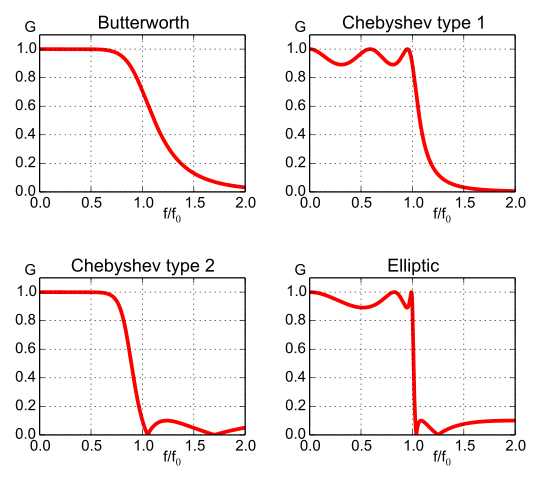
\includegraphics[width=0.6\textwidth]{./figures/FrequencyResponses.png}
    \caption{Frequency responses for different fifth order filters. \cite{Wikipedia}}
    \label{fig:FrequencyResponses}
\end{figure}

The desired cut-off frequencies were \SI{0.5}{\hertz} and \SI{100}{\hertz} for the high-pass and low-pass filters respectively. The actual values deviate from it, but the choice of resistor and capacitor pair was made by picking resistors smaller than \si{\mega\ohm} and capacitances larger than \si{\nano\farad}, that is $10^6$ and $10^{-9}$, respectively. This is so we are not working in the same order of magnitude as stray capacitances and amplifiers' internal resistances.   

The total gain needed was 1000, seeing as the ECG signal had an amplitude of around \SI{5}{\milli\volt}. In order to avoid any risk of saturation, the instrumentation and operational amplifier were given gains of 11 (due to available resistor values) and 100 respectively. No particular reason for the order, since both can achieve gain of 100 without risks.

The presence of the potential divider provides \SI{2.5}{\volt} to $V_{ref}$, allowing for use of the arduino as our single supply. There is a buffer in order to prevent loading.